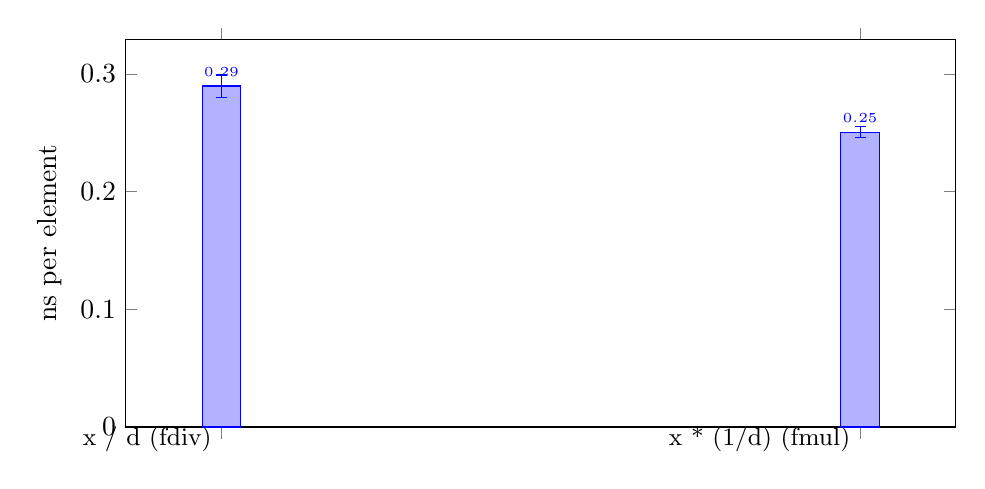
\begin{tikzpicture}
\begin{axis}[ybar, width=\textwidth, height=6.5cm, bar width=14pt, ymin=0, symbolic x coords={x / d (fdiv),x * (1/d) (fmul)}, xtick=data, x tick label style={rotate=0, anchor=east, font=\small}, ylabel={ns per element}, enlarge x limits=0.15, legend style={font=\small, at={(0.98,0.98)}, anchor=north east}, nodes near coords, nodes near coords style={font=\tiny}, every node near coord/.append style={/pgf/number format/.cd, fixed, precision=2}]
\addplot+[error bars/.cd, y dir=both, y explicit] coordinates {(x / d (fdiv),0.2897) +- (0,0.0094) (x * (1/d) (fmul),0.2506) +- (0,0.0050)};
\end{axis}
\end{tikzpicture}